


\section{Experiments}
\label{sec:experiment}
Although Section \ref{sec:Methodology} presents a theoretical analysis that validates the advantages and effectiveness of our method, we still conduct extensive experiments to demonstrate its practical performance.



\subsection{Experimental Setup}
\noindent
\textbf{Parameter Settings}.
We follow the cryptography \citep{Ruan2025haw, Couteau2022sharp} for selecting the security parameter $\lambda$ and set
$\lambda = 2^d, d \in \mathbb{Z}.$ We choose $R = \lambda + 1$. The values of $s$ and $f$ are determined according to specific types of experiments, and we set $n = kR + b$. From a practical perspective, the relationship between $s$ and $n$ is unknown. The value of $s$ needs to be specified when deploying the algorithm. $s$ does not reflect the actual number of safe models in the $\mathcal{MG}$. To cover general practical scenarios, we adopt the weakest security assumption and set $s = \lceil \frac{n+1}{2} \rceil$. This setting is similar to the widely used $3f+1=n$ in distributed systems research \citep{zhang2023waterbear, Zhang2022pace}.



\noindent
\textbf{Datasets and Models}. 
To reflect adversarial conditions in real-world scenarios, we construct the probability distribution of the safe model using the output distributions of Qwen2.5-7b-instruct, Qwen2.5-0.5b-instruct \citep{qwen2025qwen25technicalreport}, and Qwen3Guard-Gen-8B \citep{zhao2025qwen3guard} on safety evaluation datasets. The datasets include HarmBench \citep{mazeika2024harmbench} and AdvBench \citep{zou2023universal}. We generate the perturbed probability distributions of the unsafe models by referring to the probability distribution of the safe model. This process simulates $f$ Byzantine models that an adversary can fully control. 

\noindent
\textbf{Evaluation Protocol}. To reduce randomness, we report experimental results obtained from 8,000 repeated experiments.



\begin{figure*}[!]
    \centering
    \begin{subfigure}{0.32\textwidth}
        \centering
        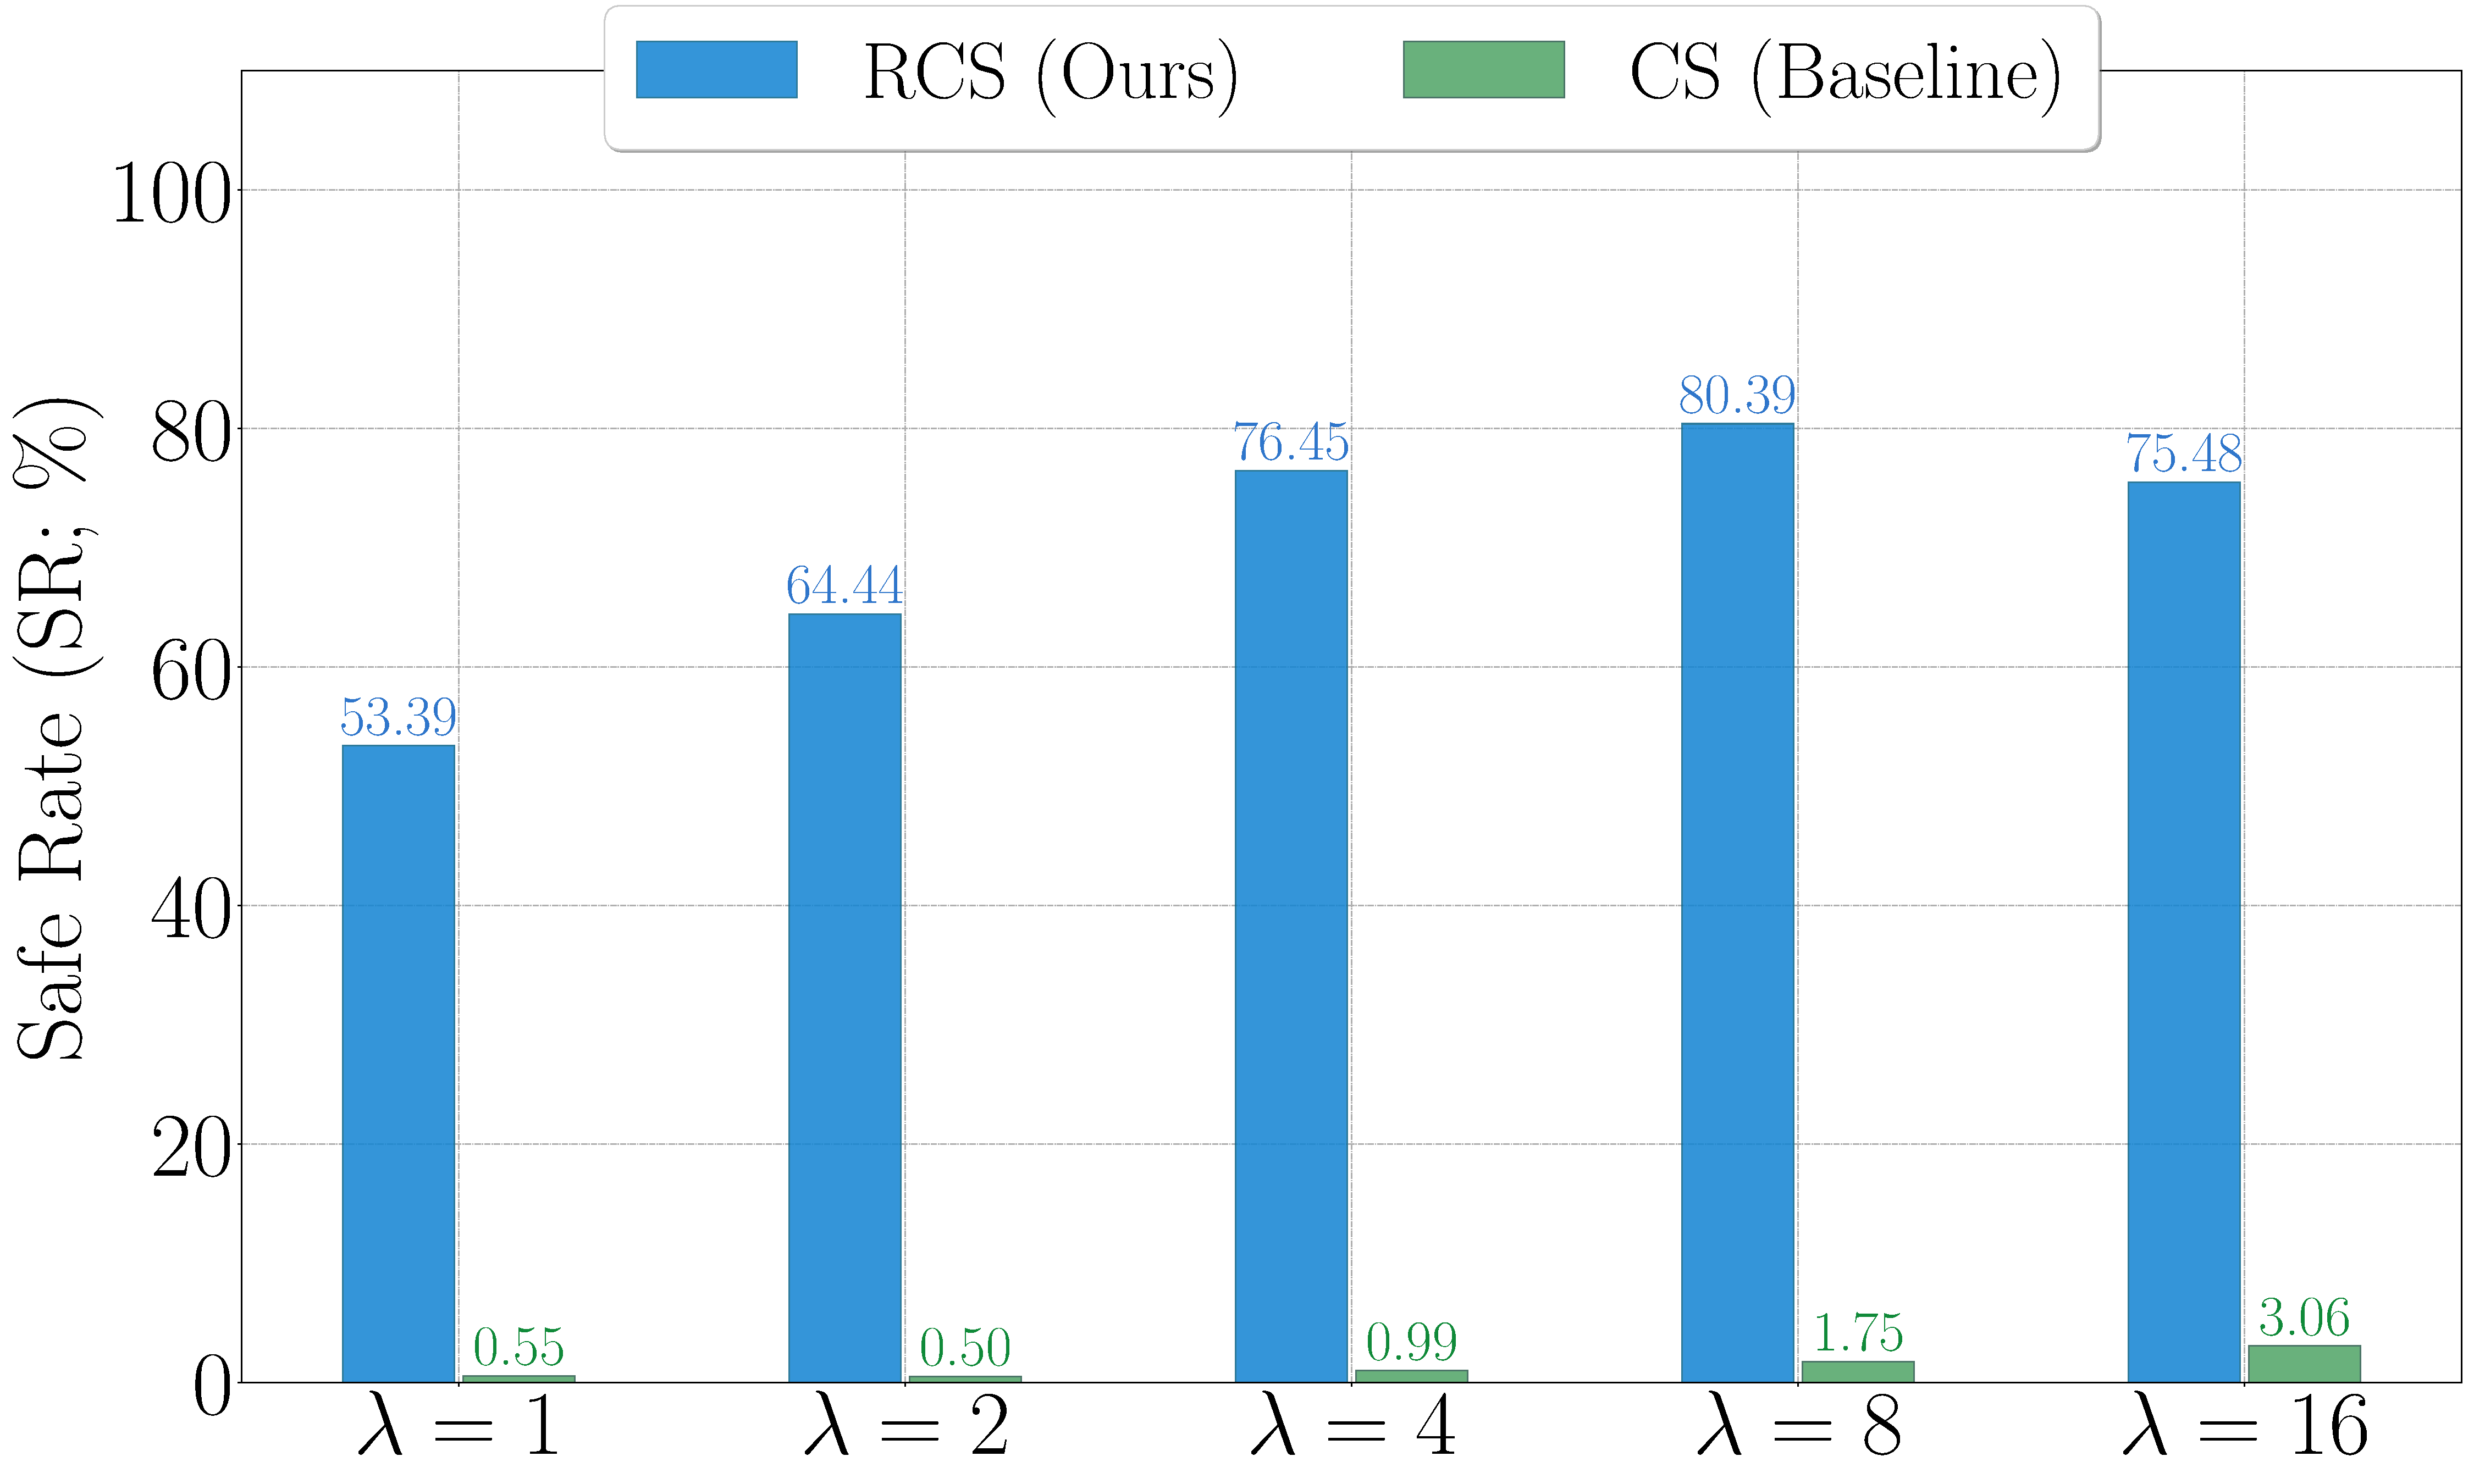
\includegraphics[width=\linewidth]{latex/eval_res_m/SR-33-m.pdf}
        \caption{$n=33$.}
    \end{subfigure}
    \begin{subfigure}{0.32\textwidth}
        \centering
        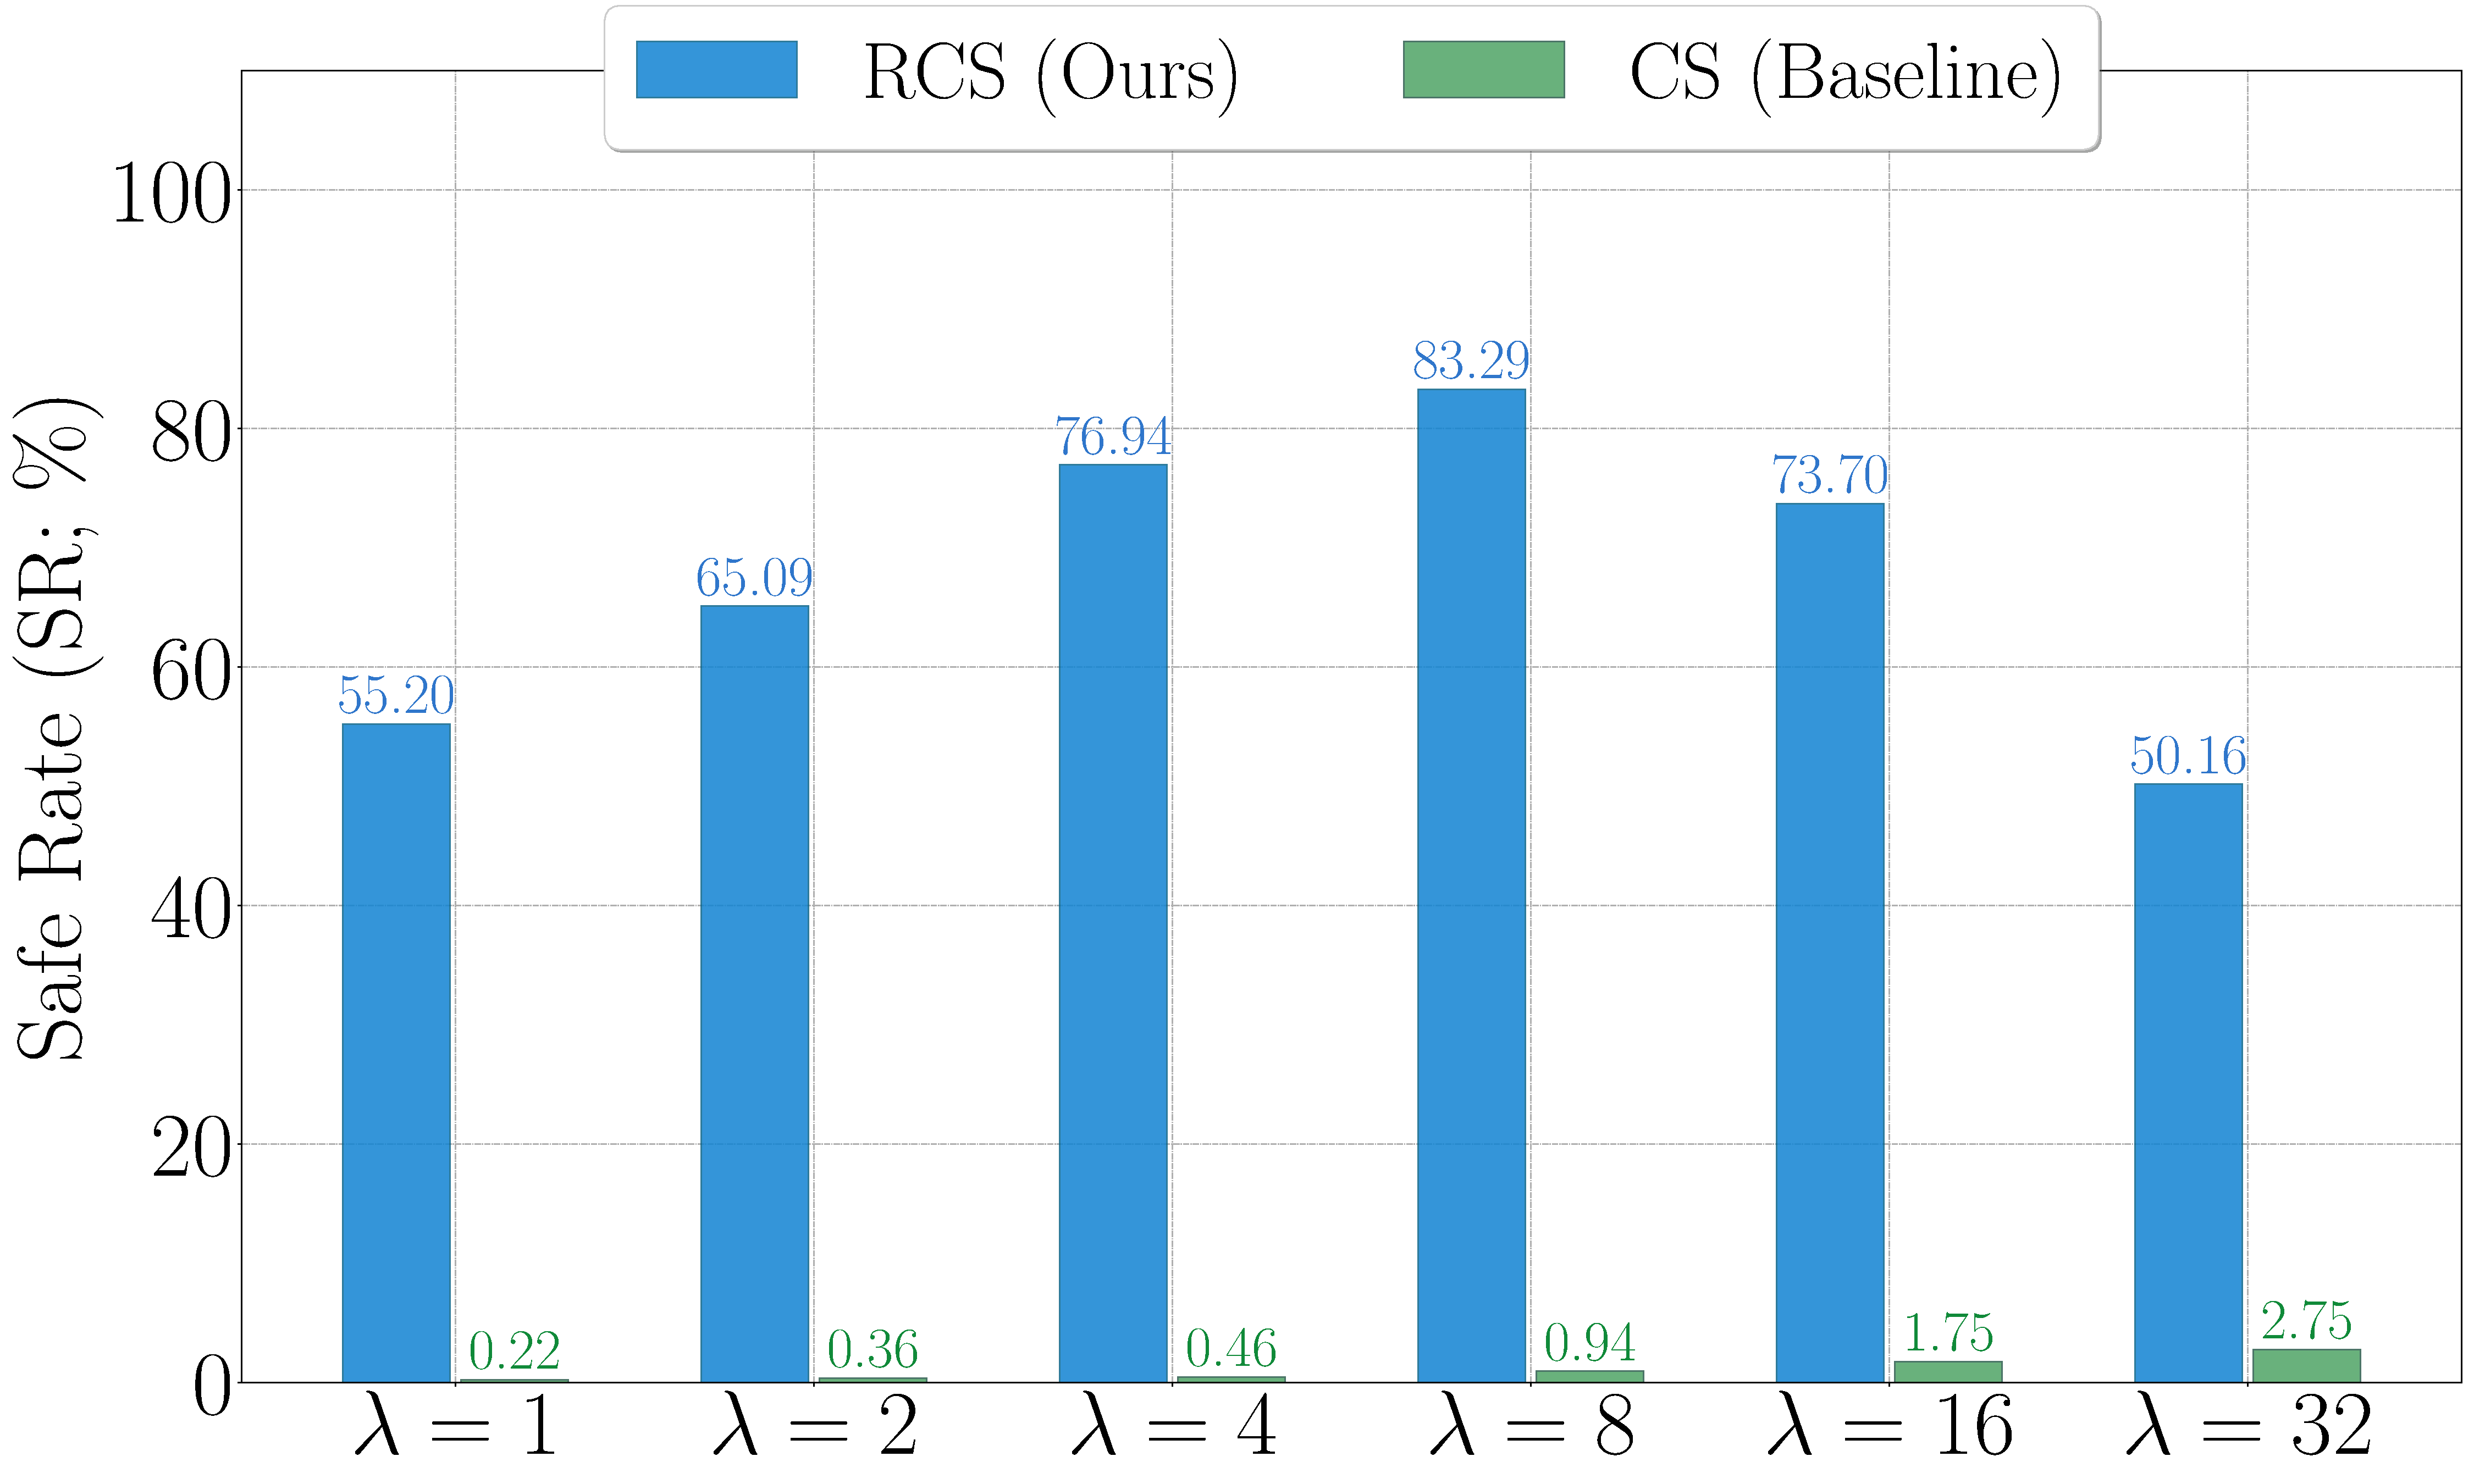
\includegraphics[width=\linewidth]{latex/eval_res_m/SR-65-m.pdf}
        \caption{$n=65$.}
    \end{subfigure}
    \begin{subfigure}{0.32\textwidth}
        \centering
        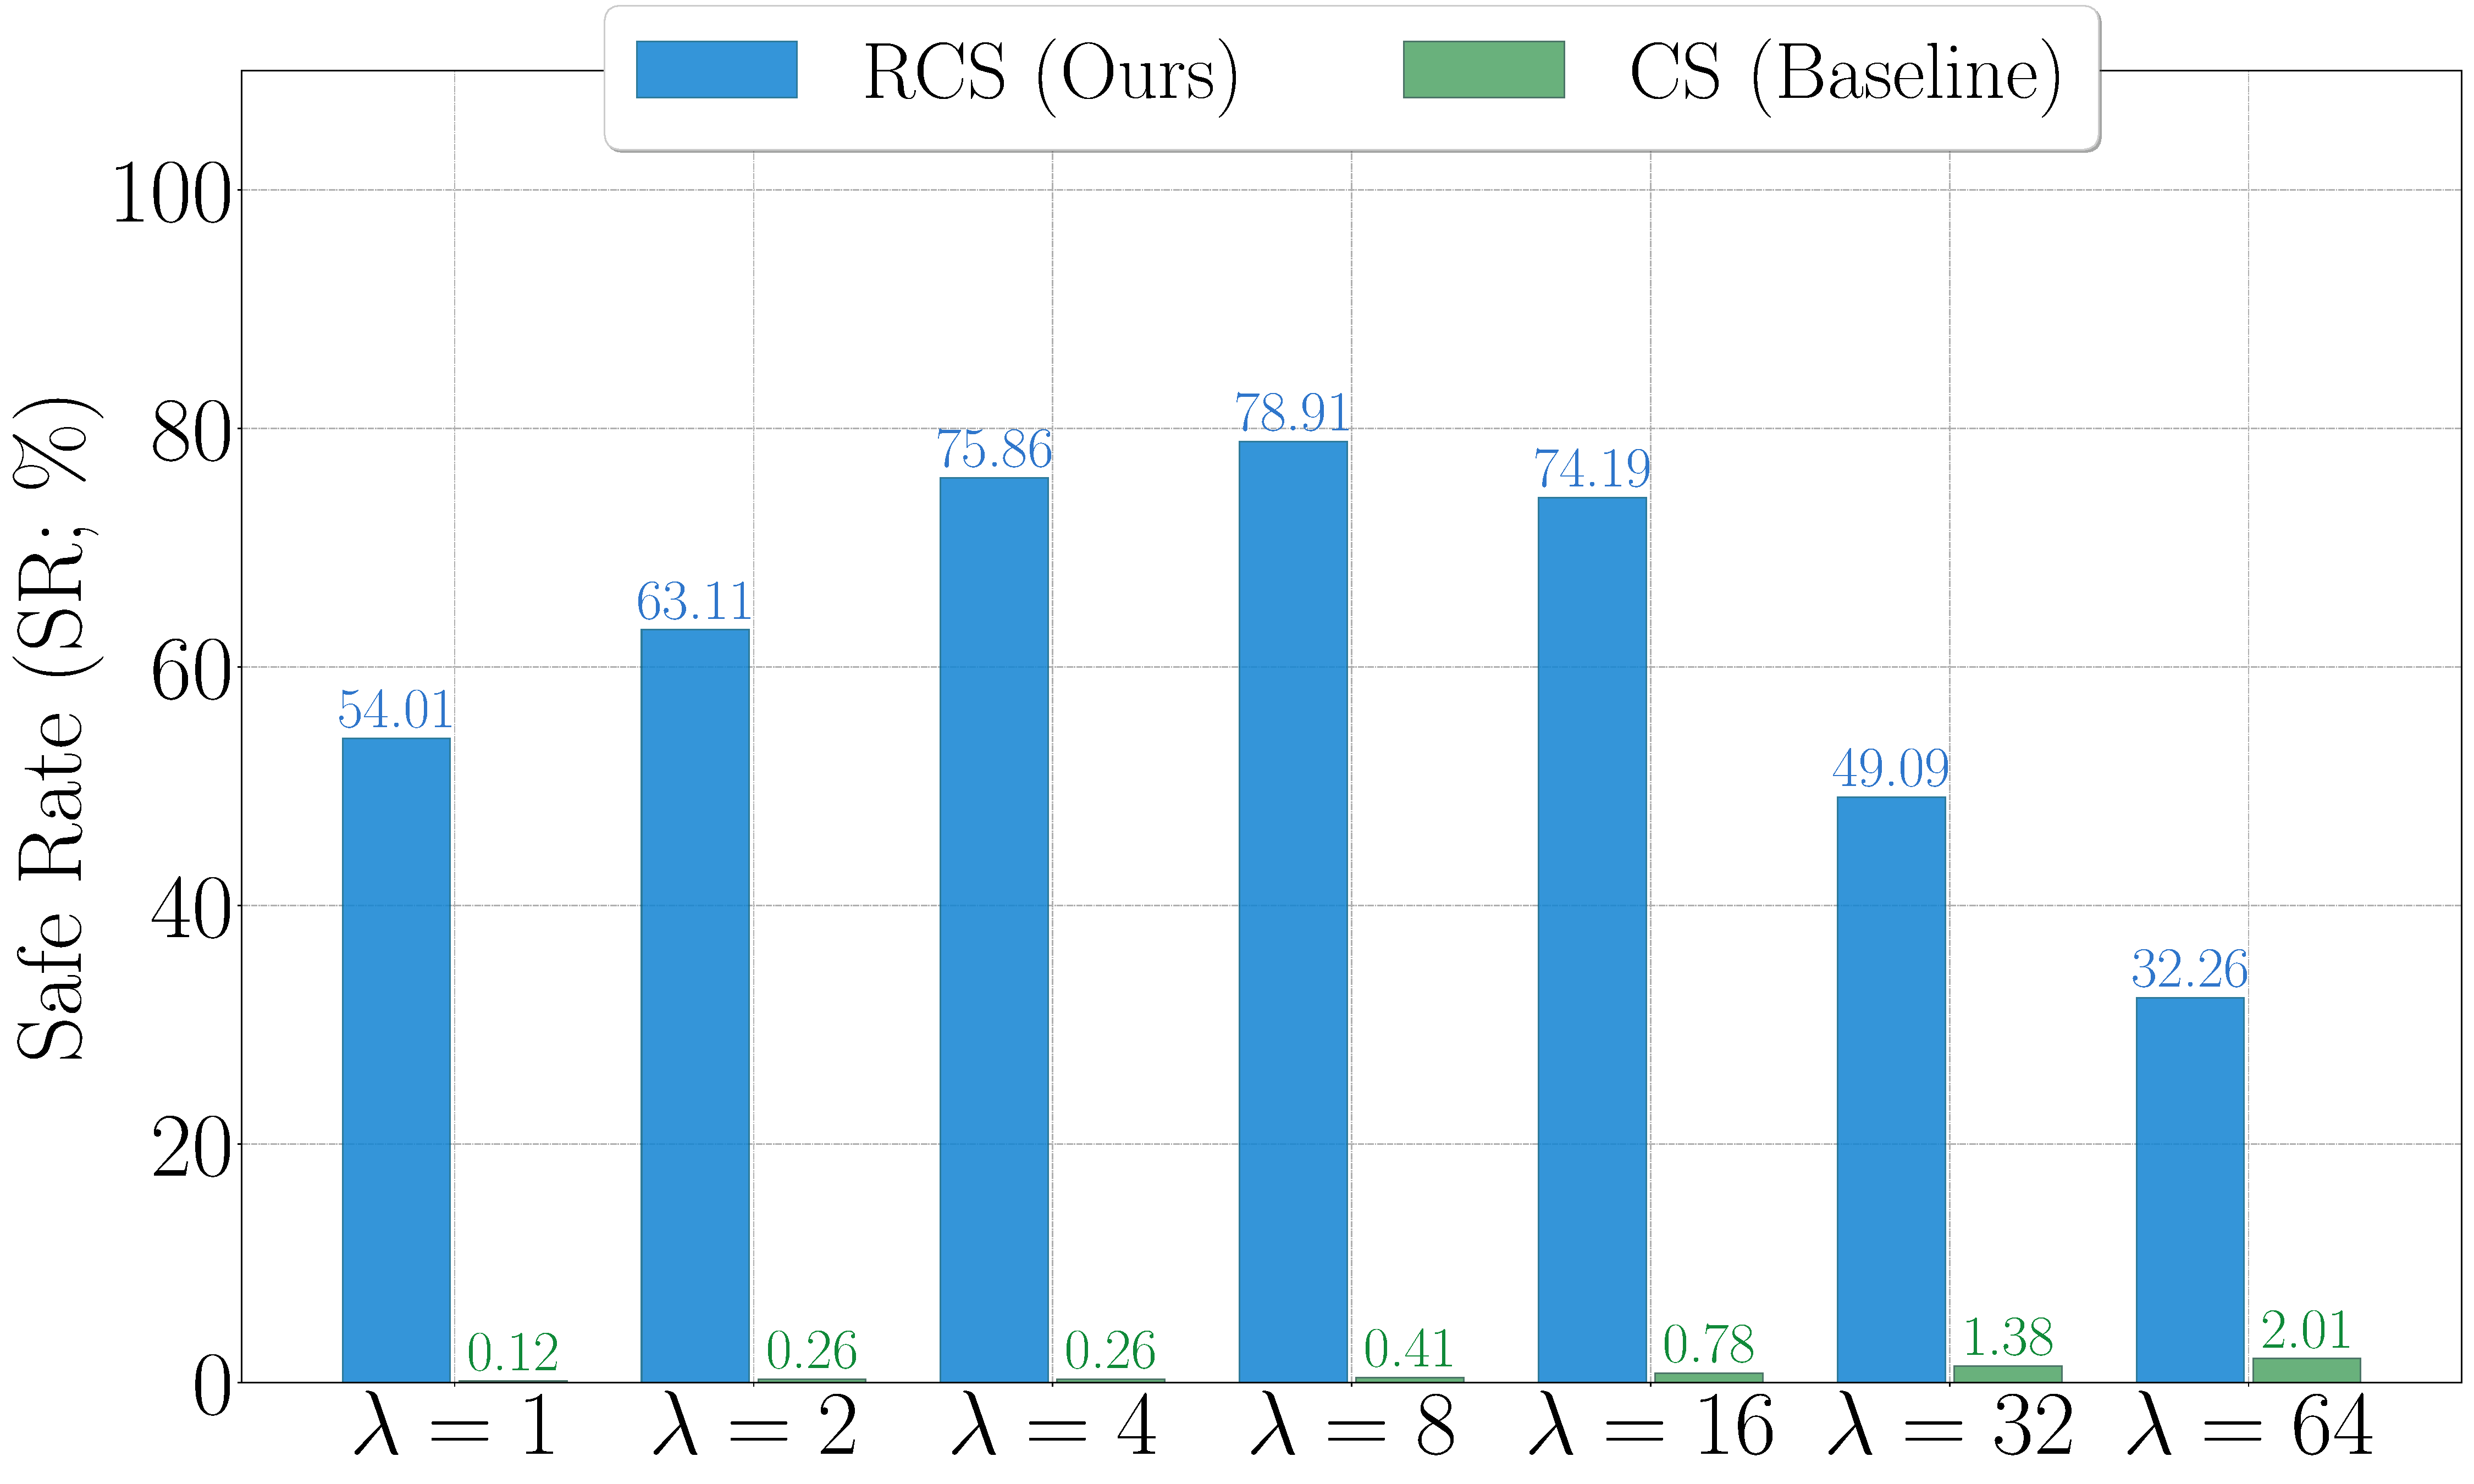
\includegraphics[width=\linewidth]{latex/eval_res_m/SR-129-m.pdf}
        \caption{$n=129$.}
    \end{subfigure}
    \caption{Evaluation results for the safe rate when Byzantine models collude.}
    \label{fig:SR_m}
    \vspace{-5pt}
\end{figure*}






\begin{figure*}[!]
    \centering
    \begin{subfigure}{0.32\textwidth}
        \centering
        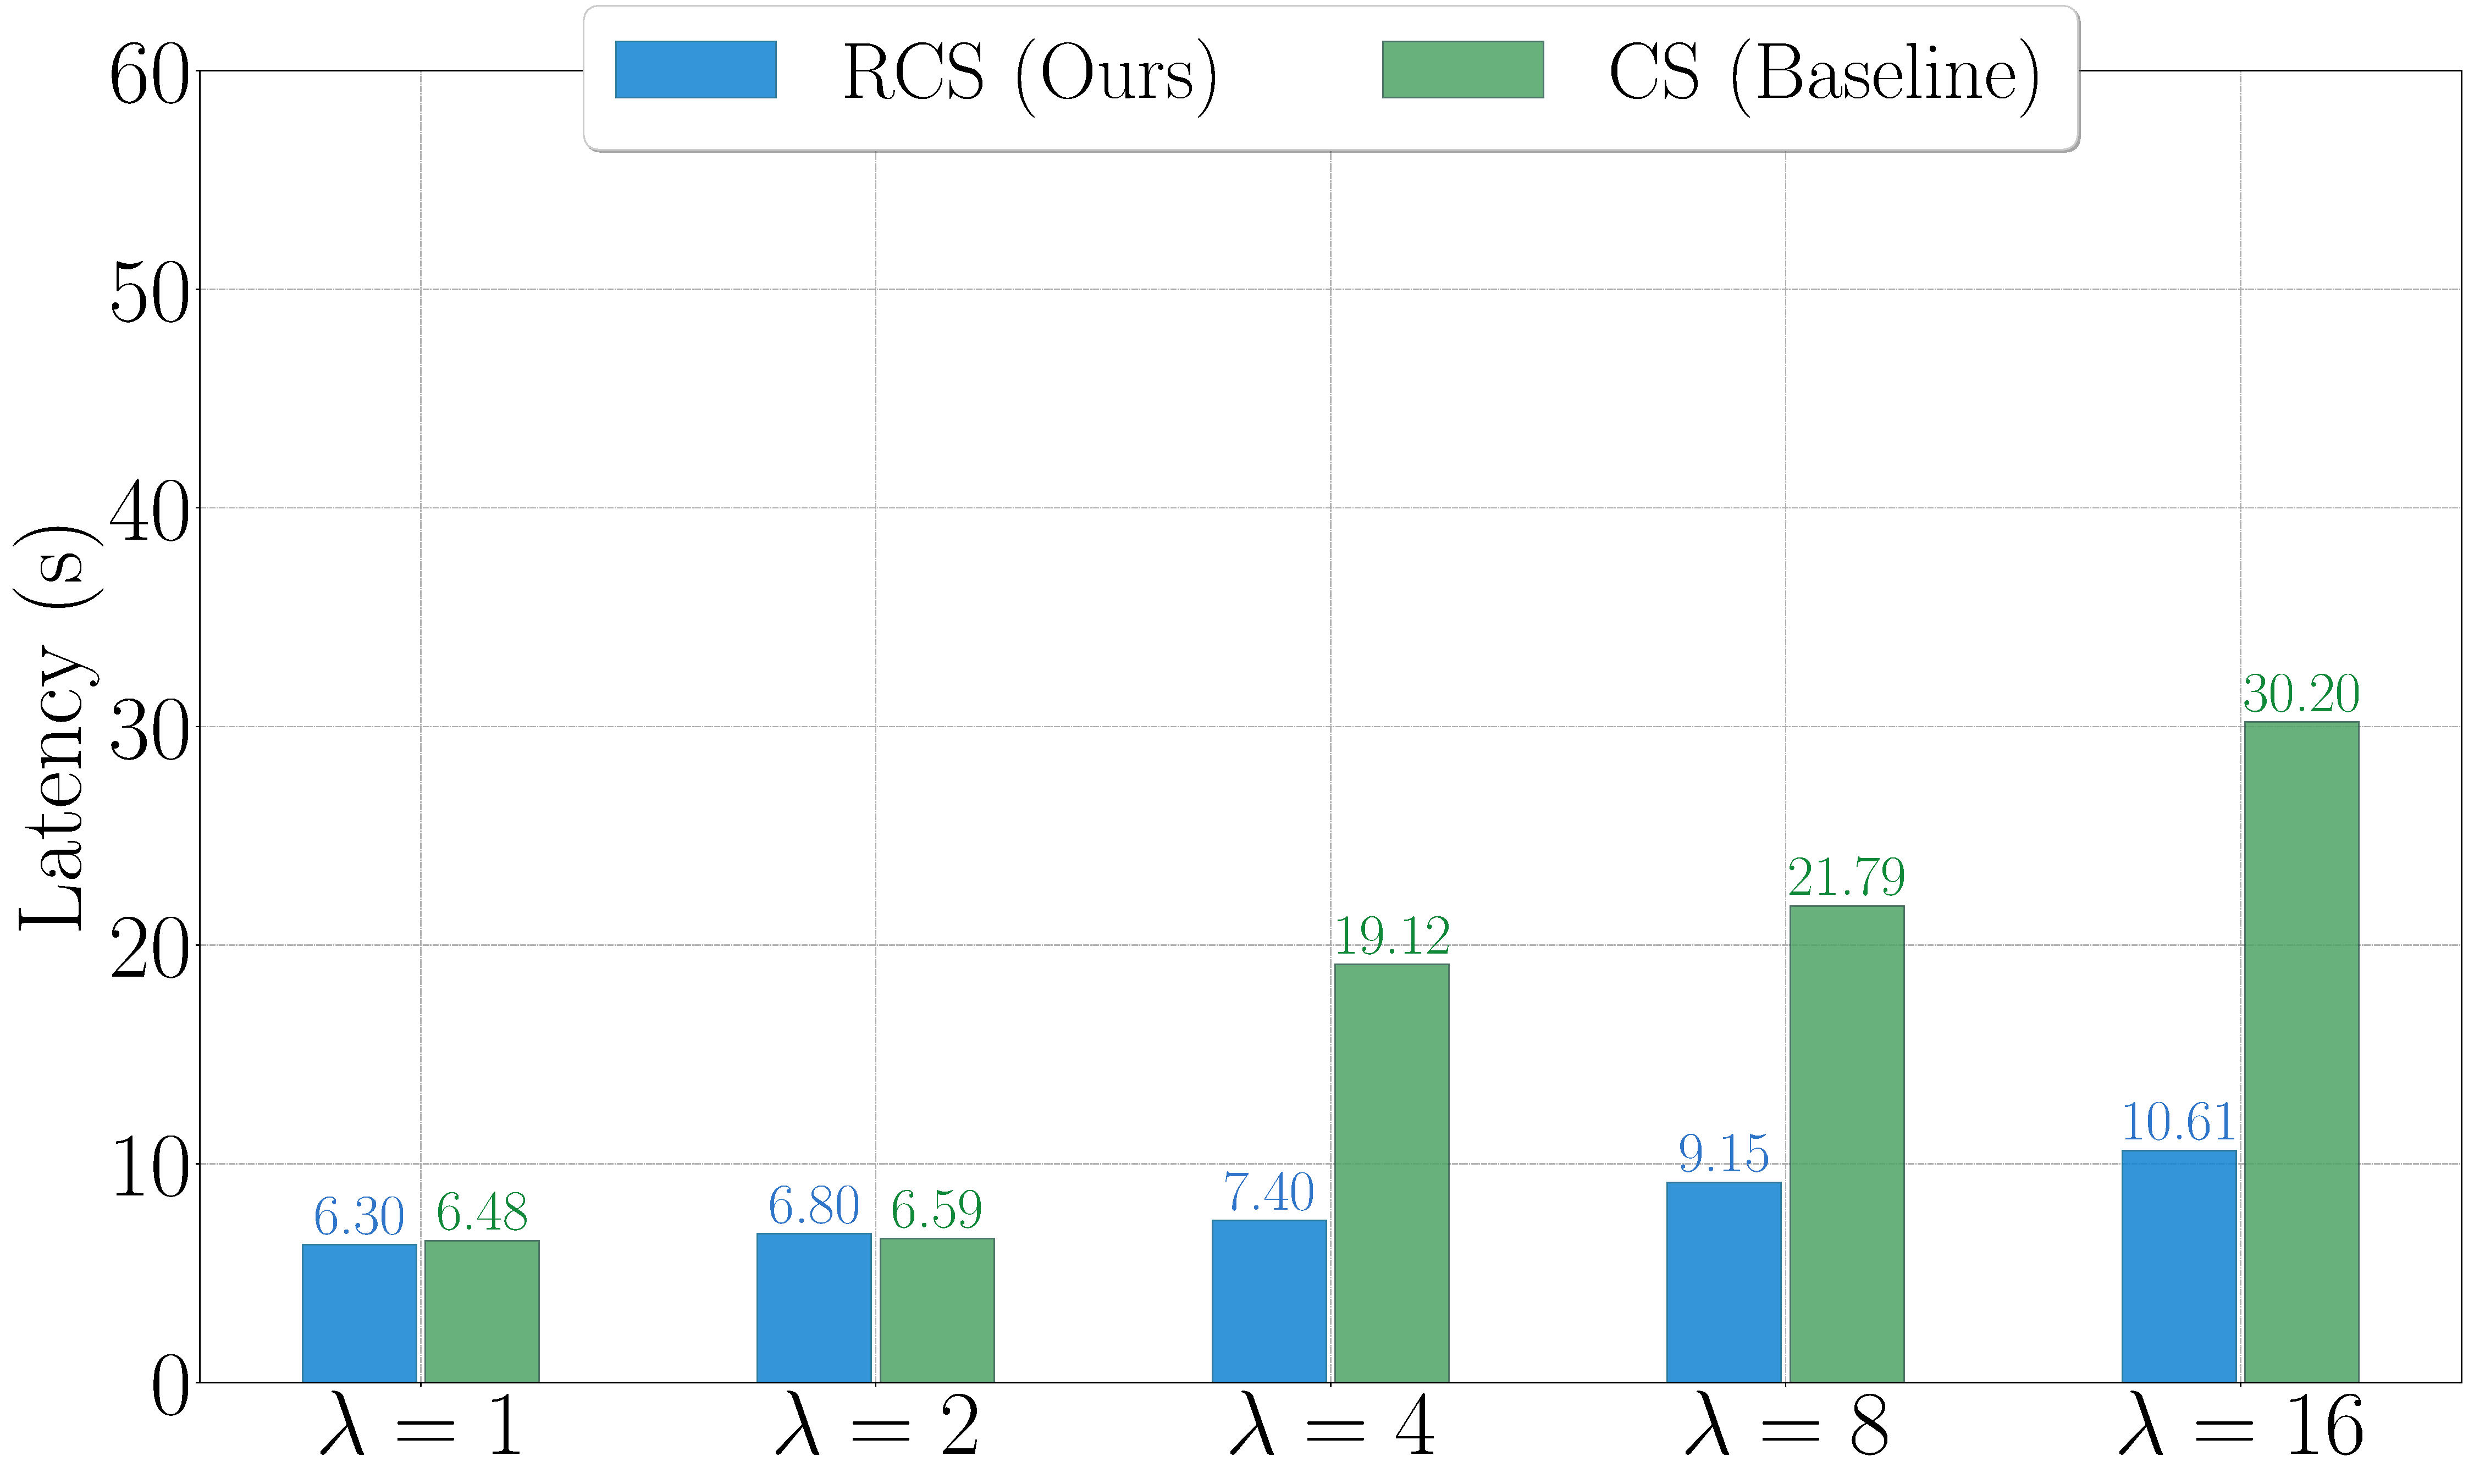
\includegraphics[width=\linewidth]{latex/eval_res_m/TC-33-m.pdf}
        \caption{$n=33$.}
    \end{subfigure}
    \begin{subfigure}{0.32\textwidth}
        \centering
        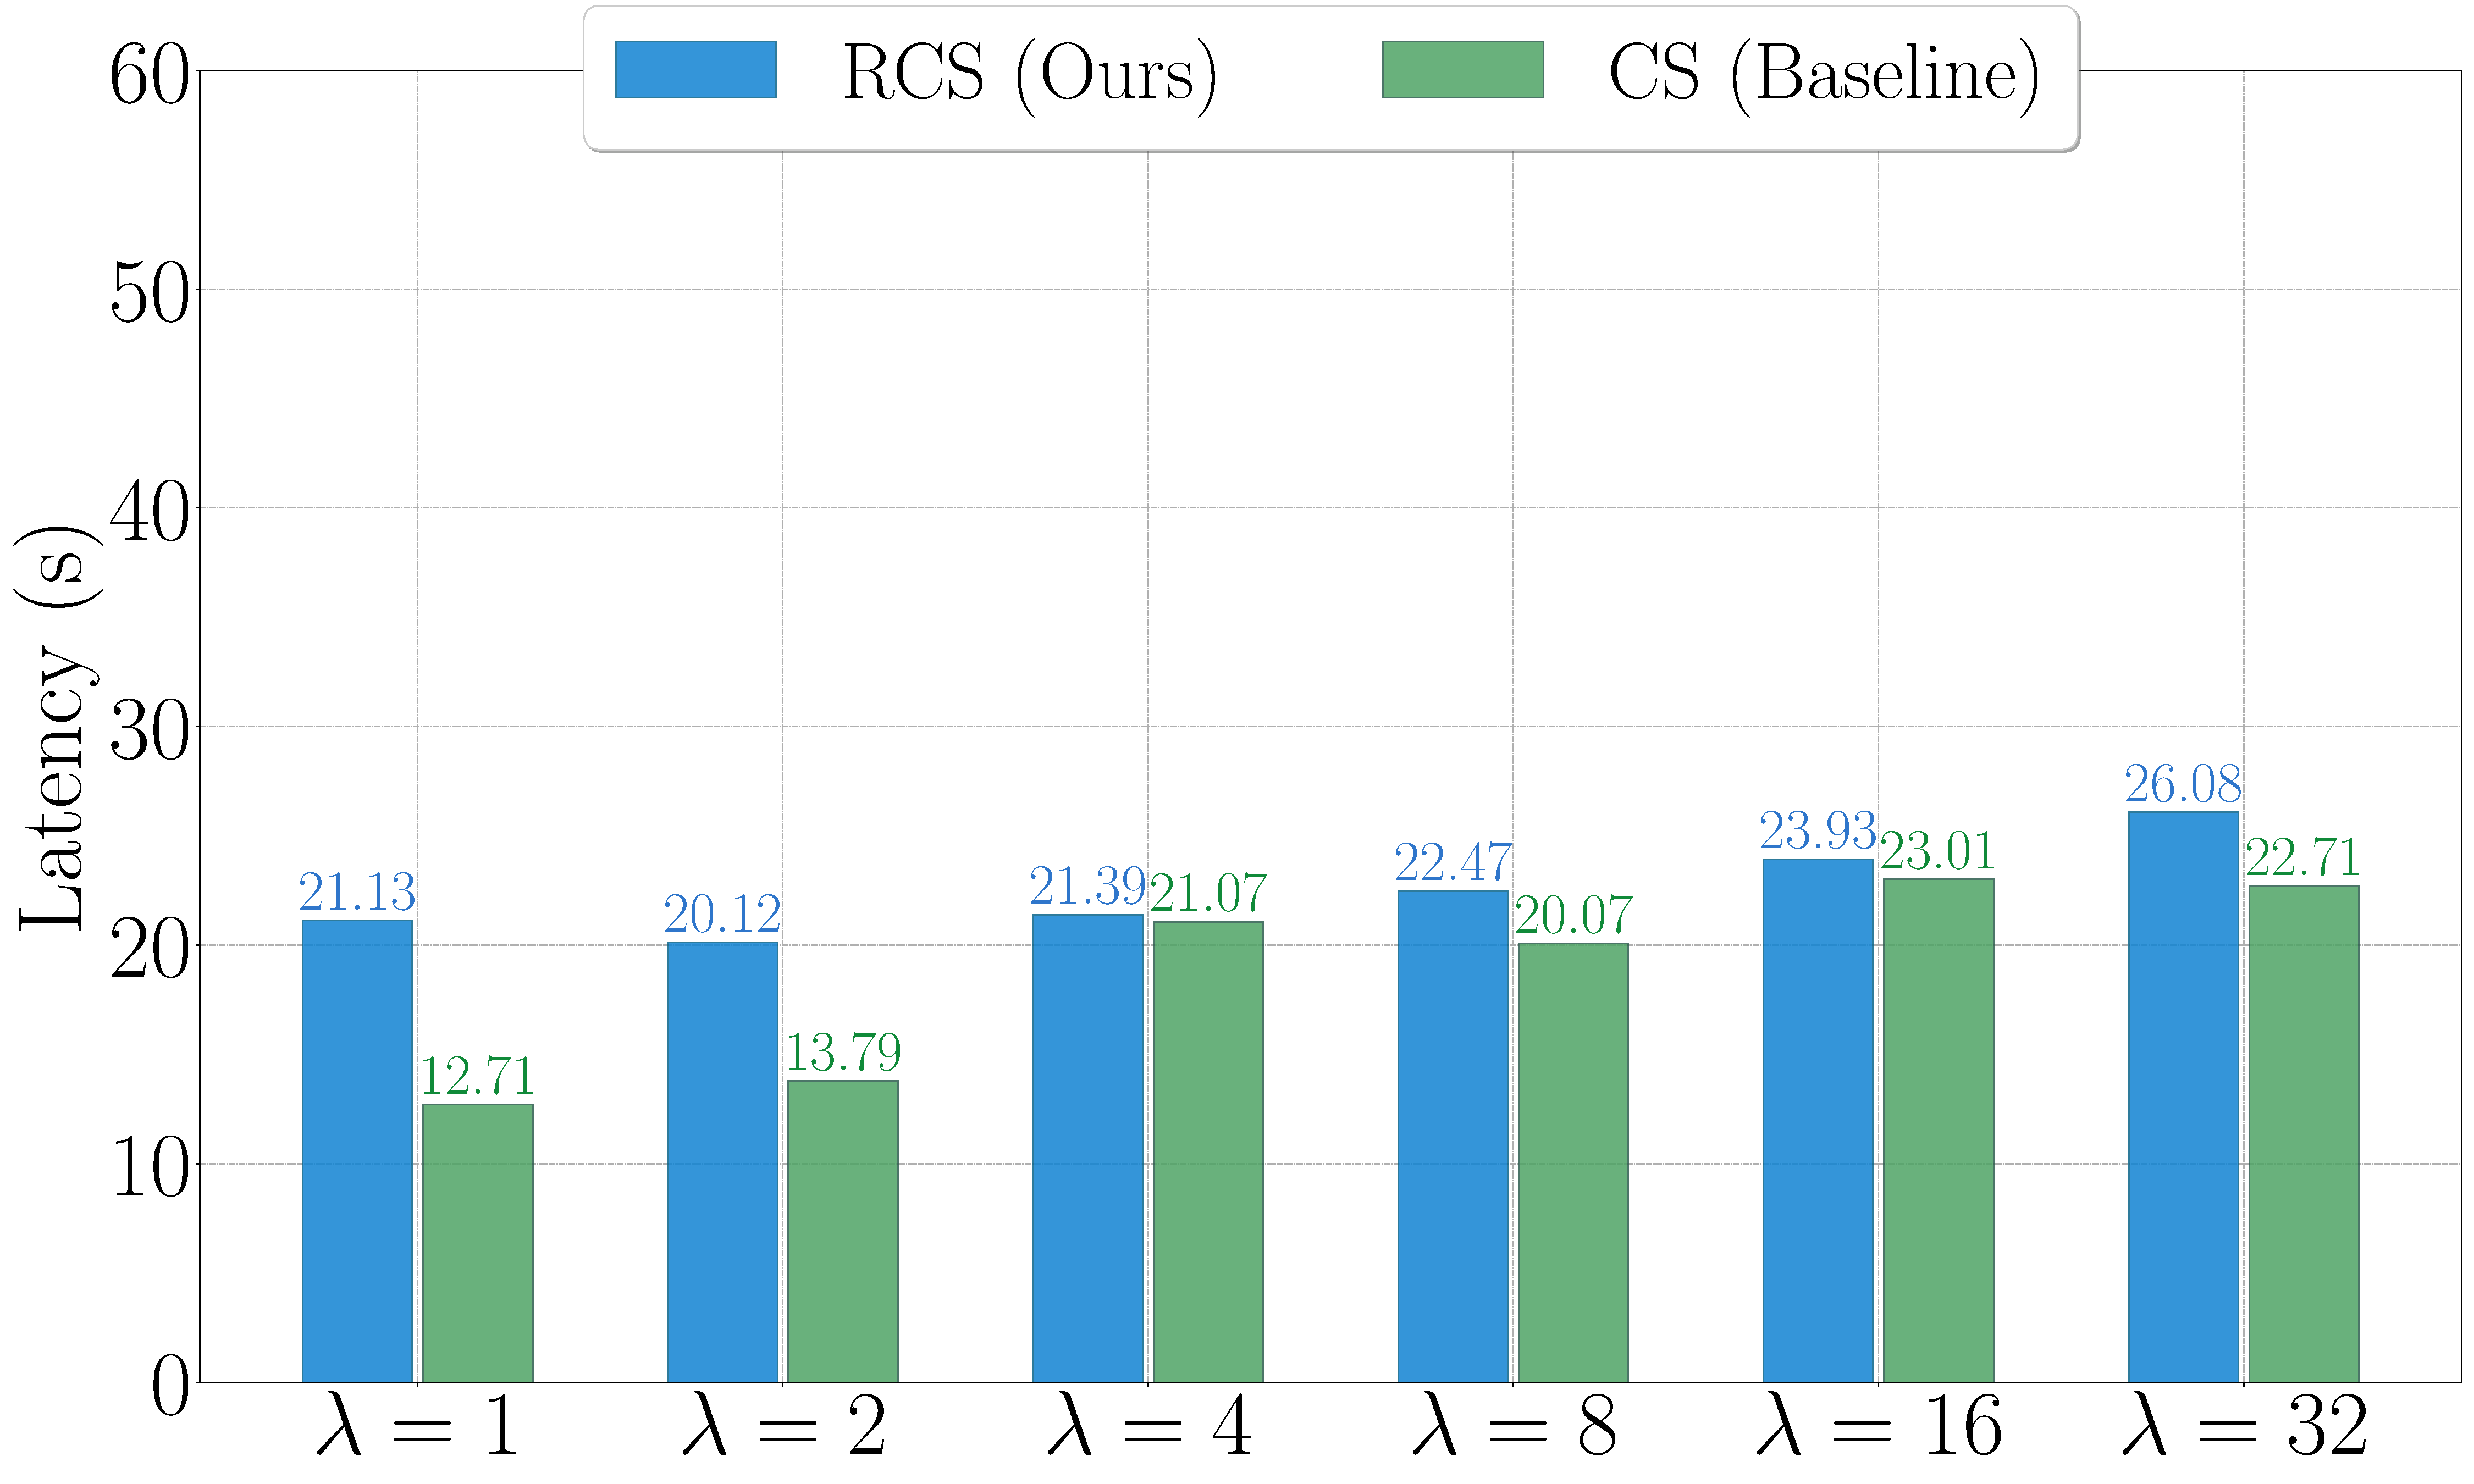
\includegraphics[width=\linewidth]{latex/eval_res_m/TC-65-m.pdf}
        \caption{$n=65$.}
    \end{subfigure}
    \begin{subfigure}{0.32\textwidth}
        \centering
        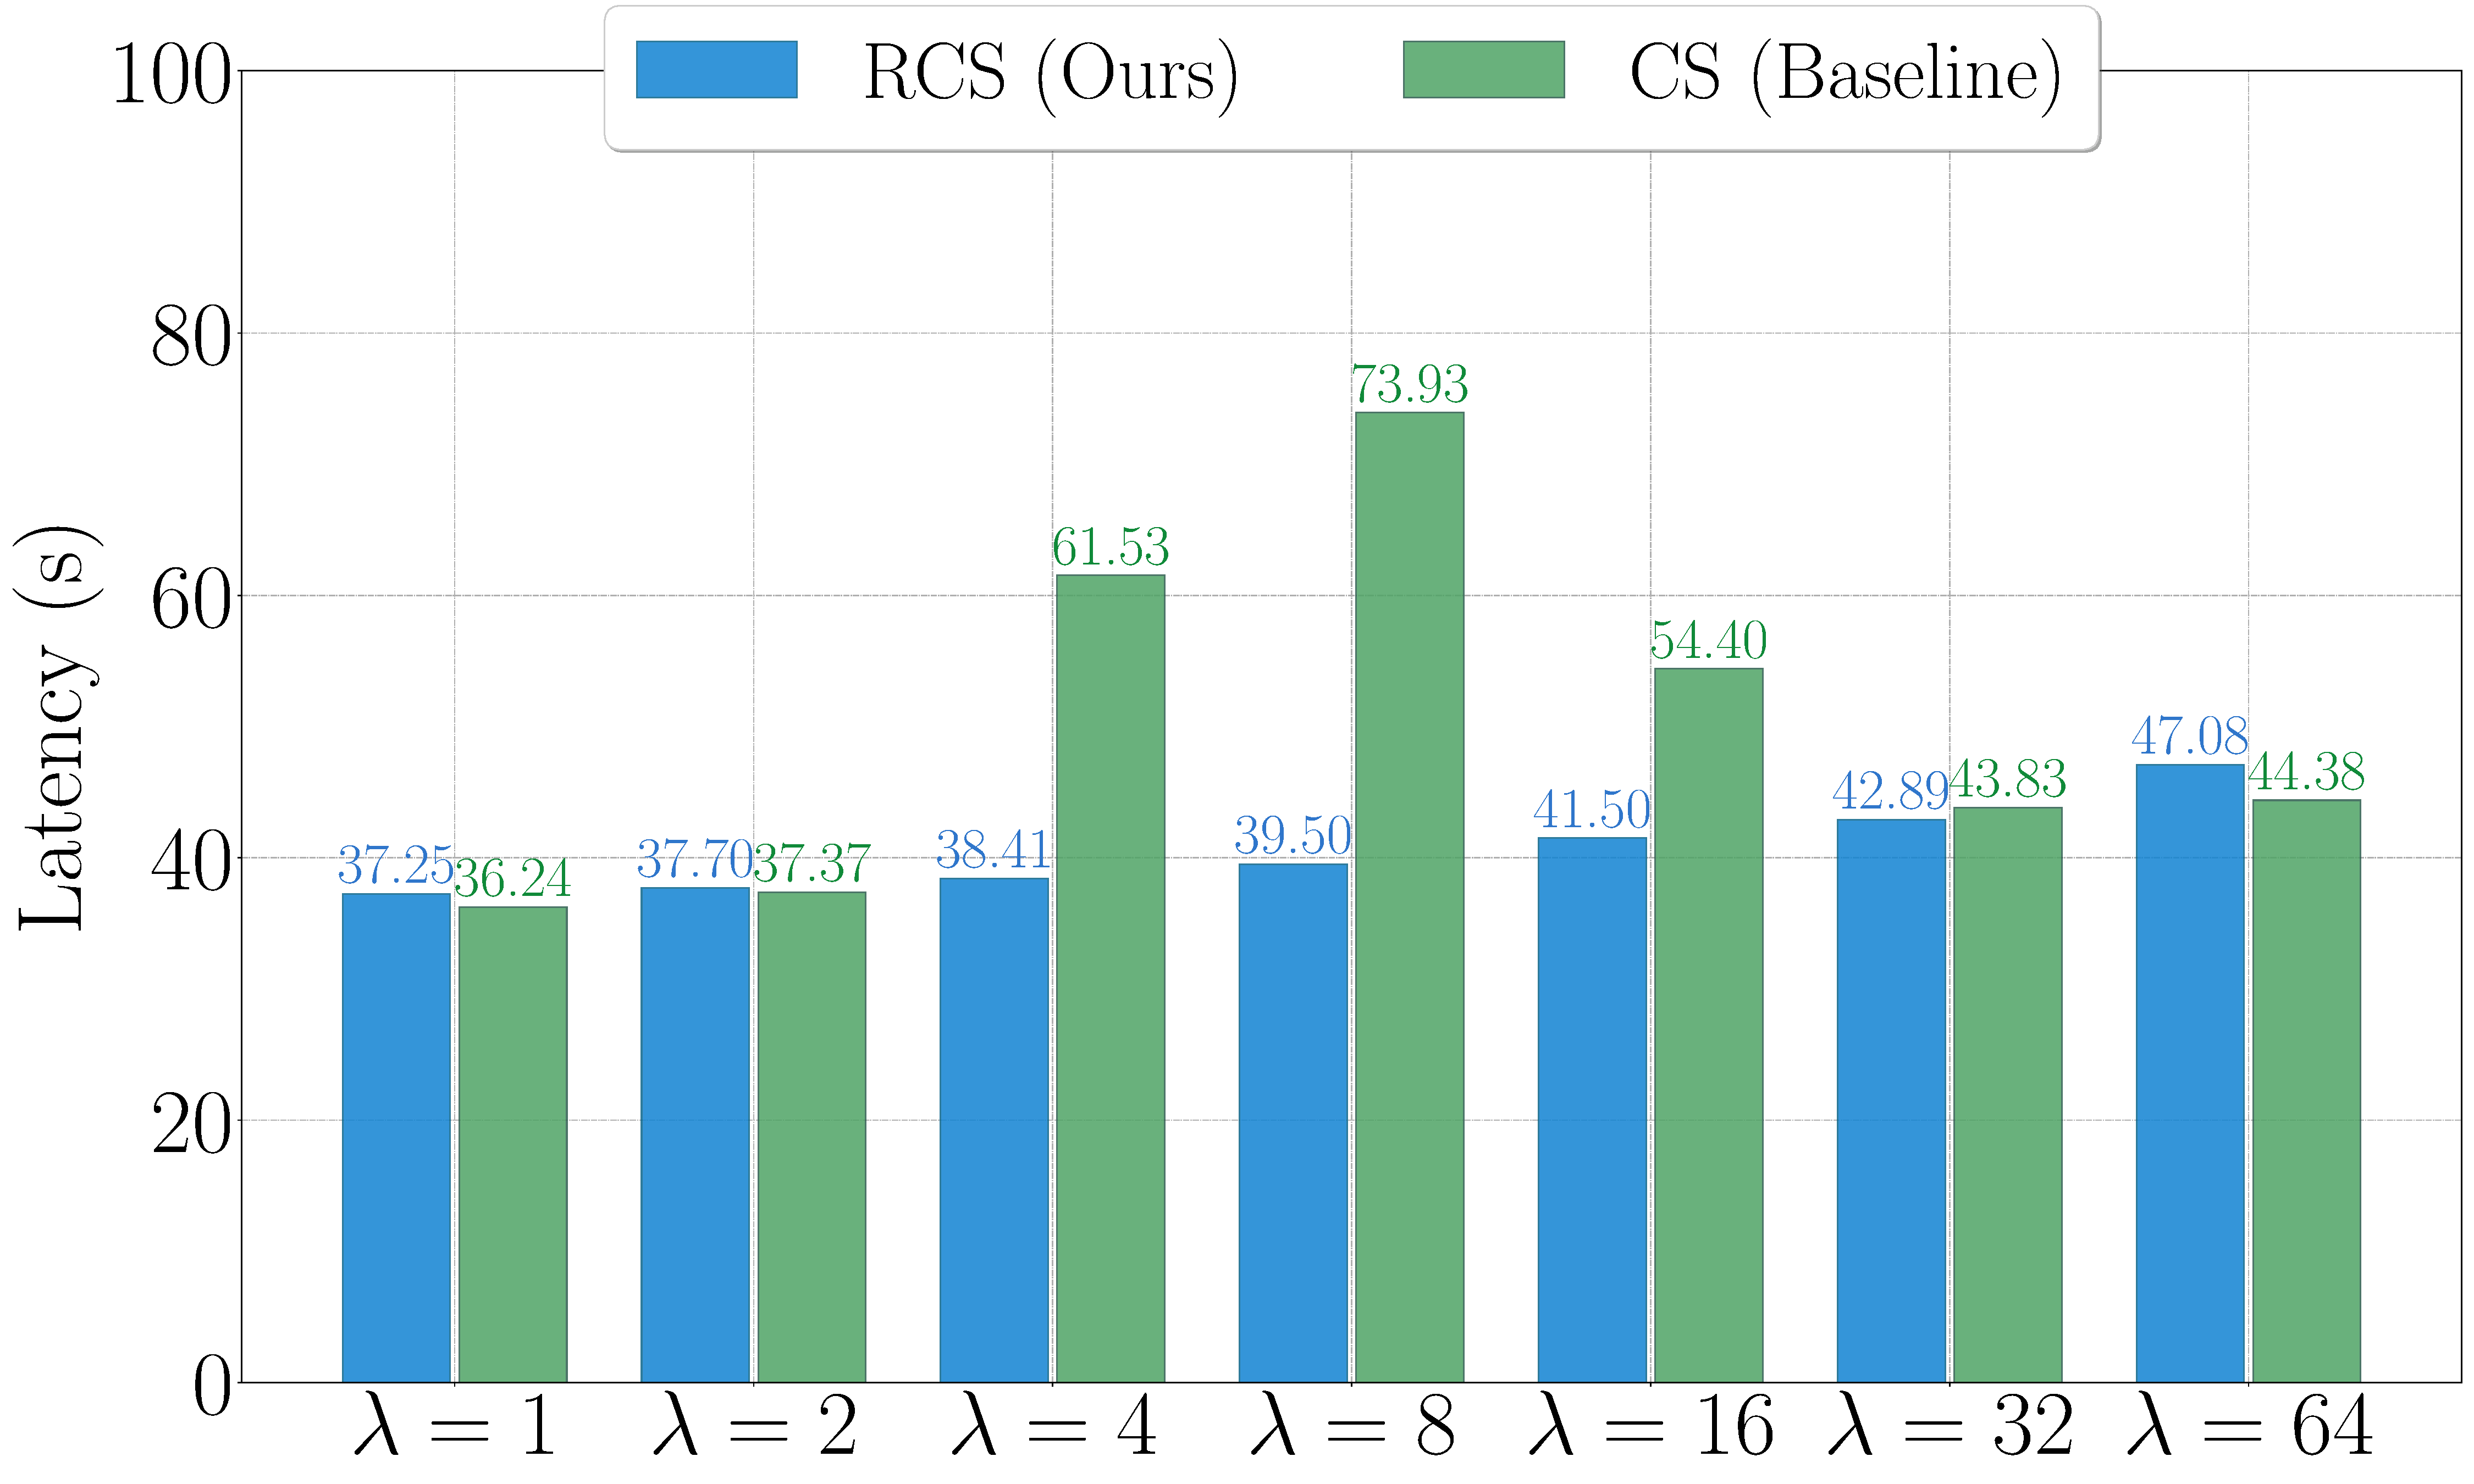
\includegraphics[width=\linewidth]{latex/eval_res_m/TC-129-m.pdf}
        \caption{$n=129$.}
    \end{subfigure}
    \caption{Evaluation results for the latency when Byzantine models collude.}
    \label{fig:TC_m}
    \vspace{-15pt}
\end{figure*}





\subsection{Evaluation Metrics}
In this work, we do not define specific criteria that label a response as safe or unsafe. For example, under jailbreak attacks, LLMs may output tokens such as "Sorry" or "Sure" \citep{wang-etal-2025-vulnerability}. These outputs reflect temporary experimental observations. They do not imply provable security in a theoretical sense. Therefore, our evaluation does not rely on the LLM-as-a-judge \citep{wei2025emoji} commonly used in prior jailbreak studies. We define the evaluation metrics as follows. Safe rate (SR) denotes the proportion of final responses produced by the safe models. Abstention rate (AR) denotes the proportion of cases where the $\mathcal{MG}$ returns $\perp$ instead of a usable response. Latency denotes the time interval from the start of the sampling to the delivery of the final response. Accuracy measures the precision of the feedback algorithm in F-RCS when identifying unsafe models, that is, the proportion of models detected by the feedback algorithm that are indeed unsafe.

\subsection{Experimental Results}
We evaluate settings where $f < \lceil \frac{n}{2} \rceil$. The results for large values of $n$ are shown in \autoref{fig:SR_g} and \autoref{fig:TC_g}. Results for smaller values of $n$ are reported in \autoref{app:results}. For different values of the security parameter $\lambda$, RCS achieves significantly higher safety than CS. RCS maintains comparable overall latency to CS. These results are consistent with the theoretical analysis and proofs in Section \ref{sec:Methodology}. CS often leads to abstention, which reduces SR. We further evaluate the algorithms under Byzantine model collusion. Results for large values of $n$ are shown in \autoref{fig:SR_m} and \autoref{fig:TC_m}. Under collusion, the safety of CS degrades catastrophically compared to the $f < \lceil \frac{n}{2} \rceil$ setting. In contrast, the safety of RCS is only slightly affected. RCS maintains more than $67\%$ safety. This result demonstrates strong resistance to collusion. To assess half-resilience, we also evaluate the case where $f = \lceil \frac{n}{2} \rceil$. The results are reported in \autoref{app:results}. In this case, CS again exhibits clear safety weaknesses and performs significantly worse than RCS. \autoref{tab:comparison} reports aggregated results across all values of $\lambda$ and $n$. RCS outperforms CS in both SR and AR. RCS also achieves comparable latency to CS. These results further validate the theoretical analysis and proofs.

For F-RCS, we evaluate the accuracy of the feedback algorithm in identifying unsafe models. The results are shown in \autoref{fig:dr} and \autoref{app:results}. We show that for different values of $\lambda$ and $n$, the average accuracy remains around 90\%. This result demonstrates the effectiveness of the feedback algorithm.



\begin{table*}[t]
\centering
\scalebox{0.87}{
    \setlength{\tabcolsep}{6pt}
    \begin{tabular}{l|llll|llll}
    \toprule
    \multirow{2}{*}{\textbf{Method}} 
    & \multicolumn{4}{c|}{\textbf{Consensus Sampling (Baseline)}} 
    & \multicolumn{4}{c}{\textbf{Reliable Consensus Sampling (Ours)}} \\
    \cmidrule(lr){2-5} \cmidrule(lr){6-9}
    & $f < \lceil \frac{n}{2} \rceil$ & $f = \lceil \frac{n}{2} \rceil$ & Collusion & AVG & $f < \lceil \frac{n}{2} \rceil$ & $f = \lceil \frac{n}{2} \rceil$ & Collusion & AVG \\
    \midrule
    Safe Rate       & 20.39 & 15.83 & 1.45  & 12.56 & 82.88 & 81.49 & 67.90 & \textbf{77.42} ($\uparrow\times 5.16$) \\
    Abstention Rate & 71.79 & 72.52 & 82.95 & 75.75 & 0.00  & 0.00 & 0.00 & \textbf{0.00} ($\downarrow 100\%$) \\
    Latency         & 22.60 & 26.73 & 21.43 & 23.59 & 24.26 & 22.21 & 18.42 & \textbf{21.63} ($\downarrow 8.31\%$) \\
    \bottomrule
    \end{tabular}
}
\caption{Comprehensive comparison between our RCS and the baseline across different dimensions. Boldface indicates the best value in each dimension.}
\label{tab:comparison}
\vspace{-10pt}
\end{table*}


\begin{figure}[t]
    \centering
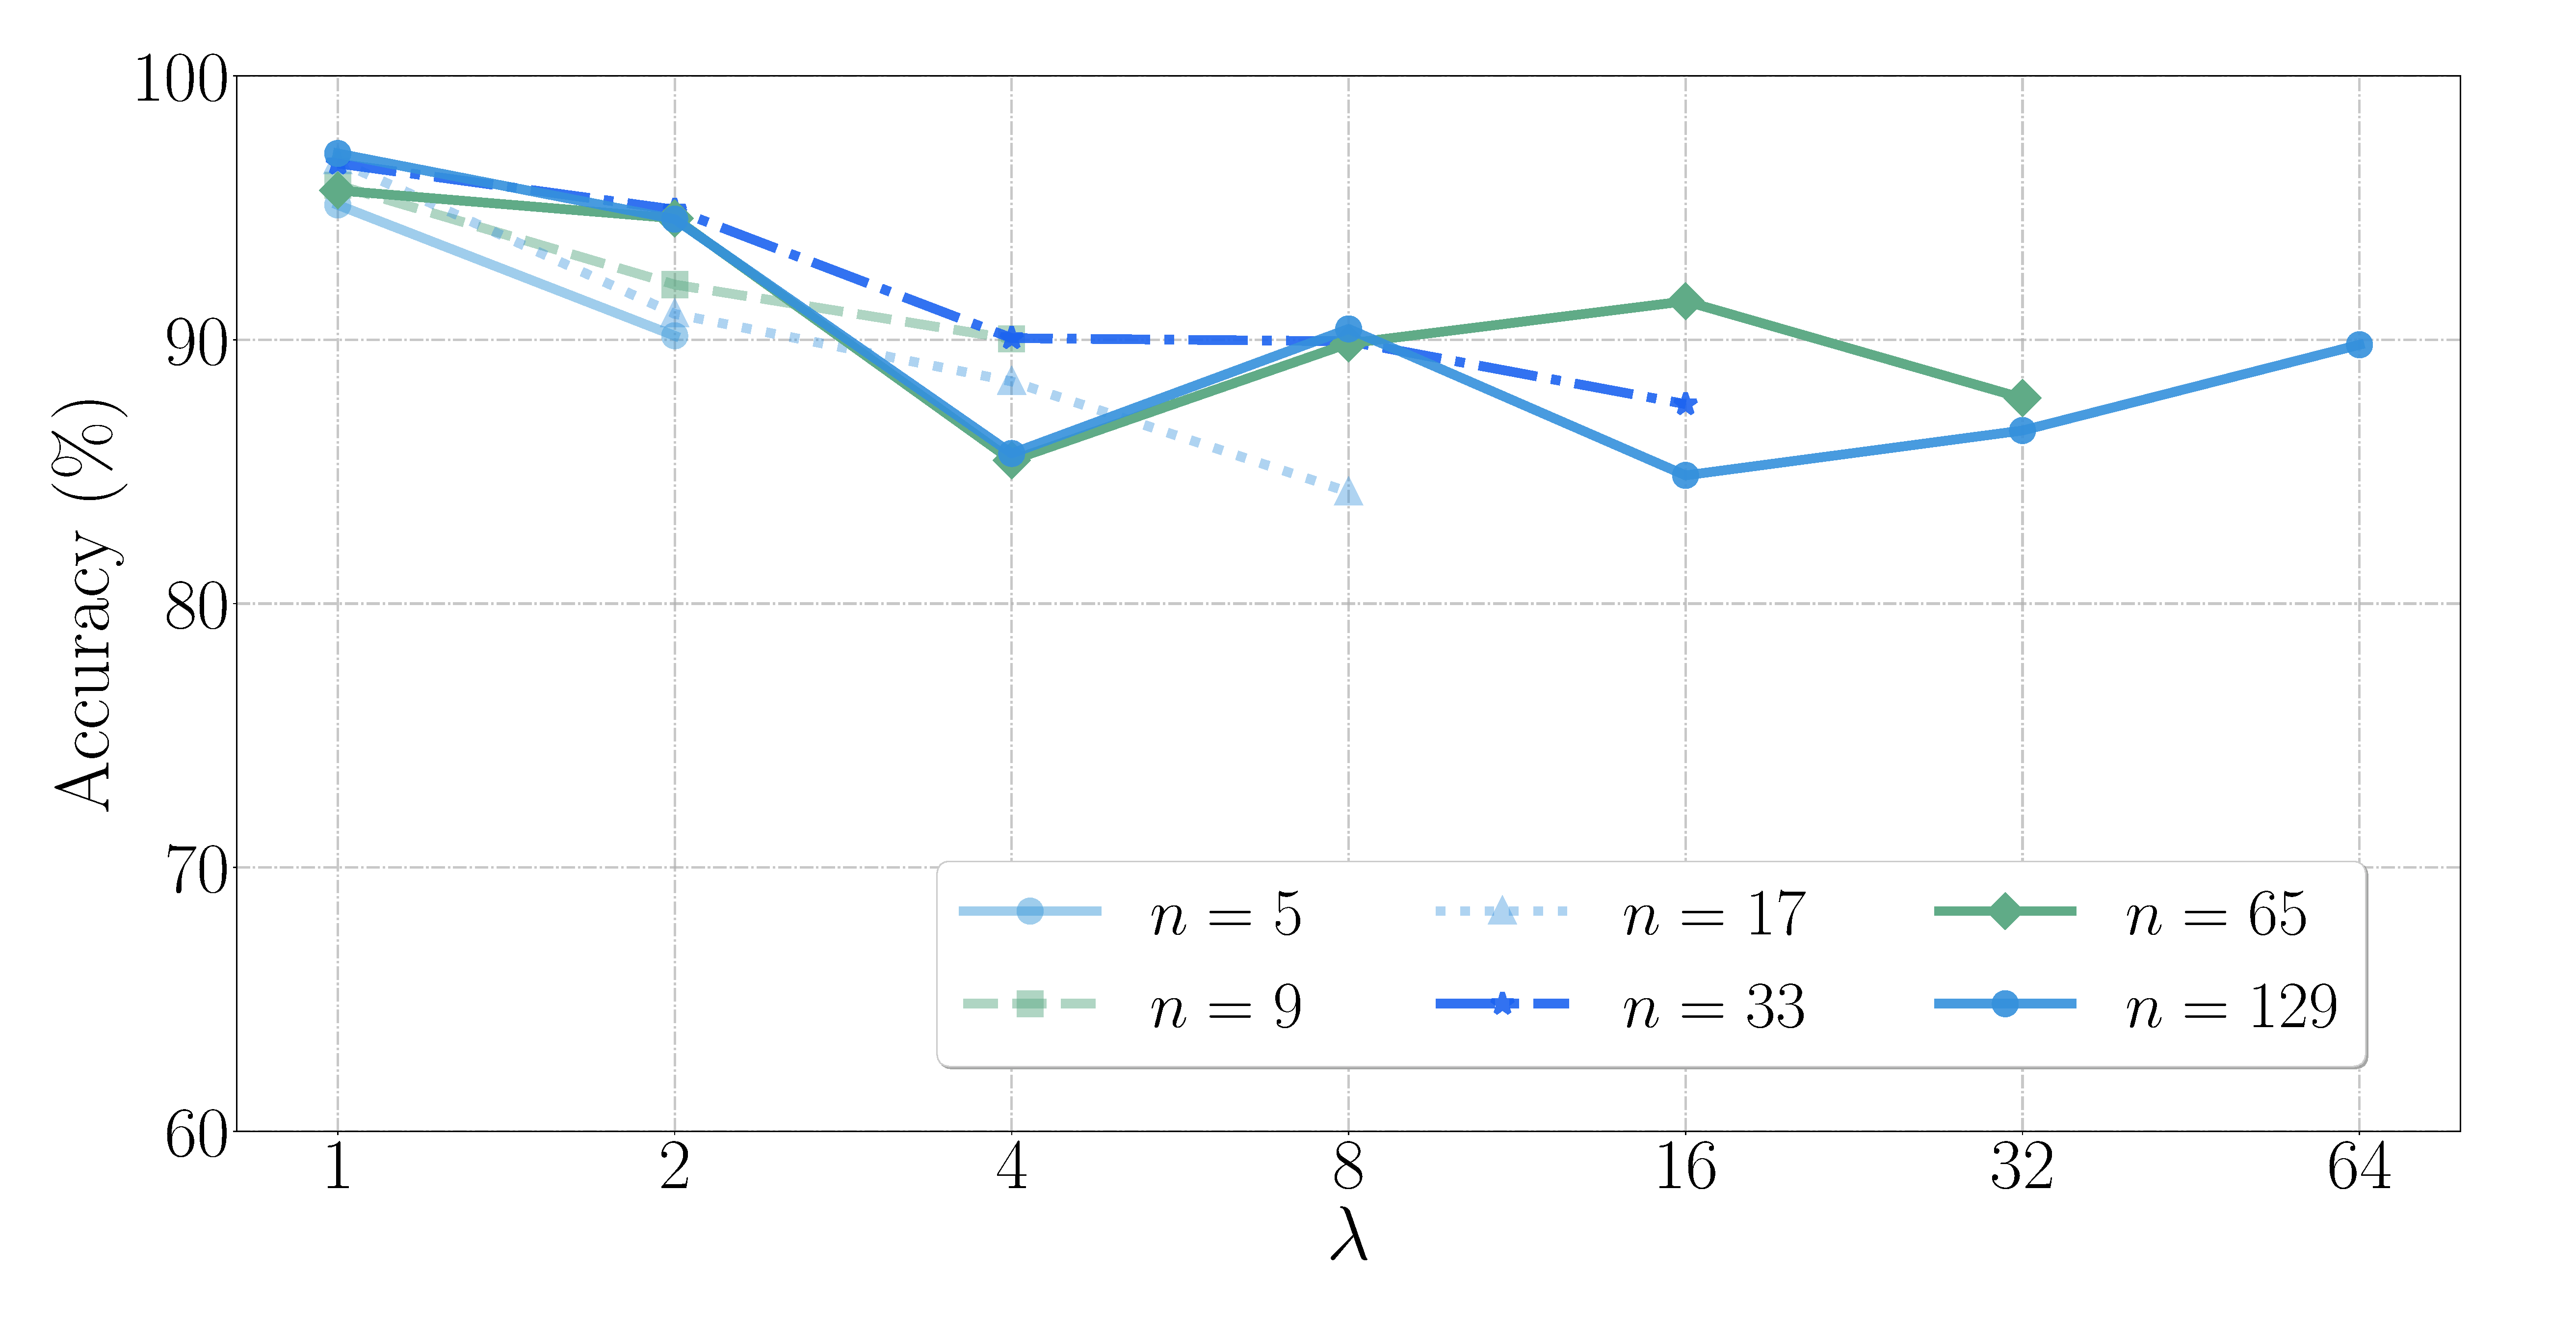
\includegraphics[width=1\linewidth]{latex/eval/DR.pdf}
    \caption{Accuracy of the feedback algorithm for different $\lambda$ and $n$ values under $f < \lceil \frac{n}{2} \rceil$.}
    \label{fig:dr}   
    \vspace{-19pt}
\end{figure}